\RequirePackage{plautopatch} % pLaTeX / upLaTeX / LuaTeX-ja の不具合修正など
\documentclass[a4paper,10pt]{ltjsarticle}
\renewcommand{\baselinestretch}{1.05}
\usepackage{luatexja}        % LuaTeX-ja で日本語を扱う

% -------------------------------
% フォント関連の設定
% -------------------------------
\usepackage{luatexja-fontspec}

% -------------------------------
% 数式・数理フォントパッケージ
% -------------------------------
\usepackage{amsmath}
\usepackage{amssymb}          % \mathbb などを使用可能に

% -------------------------------
% 図を生成するためのパッケージ
% -------------------------------
\usepackage{tikz}
\usepackage{pgfplots}
\pgfplotsset{compat=newest}

% -------------------------------
% よく使われるパッケージ群
% -------------------------------
\usepackage{geometry}
\usepackage{multicol}
\usepackage{titlesec}
\usepackage{tocloft}
\usepackage[compatibility=false]{caption}
\usepackage{flushend}
\usepackage{graphicx}
\usepackage{here}
\usepackage{multirow}
\usepackage{threeparttable}
\usepackage{tabularx}  % 重複削除済み
\usepackage{enumitem}
\usepackage{url}
\usepackage{subcaption}  % subfig の代わりにこれを使用
\usepackage{indentfirst}


% -------------------------------
% 用紙余白等の設定
% -------------------------------
\geometry{
  top=20mm,
  bottom=20mm,
  left=20mm,
  right=20mm
}

\setlength{\baselineskip}{14pt}  % 行間

% -------------------------------
% タイトルやセクション見出しのフォーマット
% -------------------------------
\titleformat{\section}
  {\large\bfseries}
  {\thesection.}
  {1\zw}{}

\titleformat{\subsection}
  {\large\bfseries}
  {\thesubsection.}
  {1\zw}{}

\titleformat{\subsubsection}
  {\large\bfseries}
  {\thesubsubsection.}
  {1\zw}{}

\titlespacing*{\section}{0em}{1em}{1em}
\titlespacing*{\subsection}{0em}{1em}{1em}
\titlespacing*{\subsubsection}{0em}{1em}{1em}

% -------------------------------
% 目次の設定
% -------------------------------

\setcounter{tocdepth}{3}          % 目次の深さ
\makeatletter
\renewcommand{\numberline}[1]{#1.~}
\renewcommand{\cftsecleader}{\cftdotfill{\cftdotsep}}
\renewcommand{\cftsubsecleader}{\hfill}
\renewcommand{\cftsubsubsecleader}{\hfill}
\cftpagenumbersoff{subsection}
\cftpagenumbersoff{subsubsection}
% (例) section, subsection, subsubsection のインデントを調整
\cftsetindents{section}{0em}{5em}
\cftsetindents{subsection}{1em}{5em}
\cftsetindents{subsubsection}{1.5em}{5em}
\makeatother

% キャプション(図表の見出し)フォントサイズ設定
\DeclareCaptionFont{designatedFont}{\fontsize{10.5pt}{14pt}\selectfont}
\captionsetup{font=designatedFont}

% -------------------------------
% タイトル情報
% -------------------------------
% \title{サンプル論文タイトル}
% \author{山田 太郎}
% \date{\today}


\begin{document}

% \maketitle
% \thispagestyle{empty}
% \clearpage

\tableofcontents
\thispagestyle{empty}



% ******************************************************
% 1. はじめに
% ******************************************************
\clearpage
\setcounter{page}{1}

\section{はじめに}

近年,無線通信端末の利用者が急増し,さまざまな場所で無線通信システムが利用されている.今後もさらなる利用拡大と機能高度化が見込まれる一方,無線通信技術の進歩に伴いシステムが高機能化・複雑化している一方で,研究開発では各レイヤごとに検討が行われている.


しかし,単一レイヤでの評価では通信システム全体の性能を十分に把握することができない.

本研究では,無線通信全体の品質を総合的に評価するために,実環境の電波伝搬特性を考慮した物理層とMAC(Medium Access Control)層が連携したシミュレータの開発の一環として,IEEE 802.11規格に基づくCSMA/CA(Carrier Sense Multiple Access with Collision Avoidance)方式を用いたMAC層の挙動をする無線LAN(Local Area Network)モデルを開発し,その有効性を評価することを目指す.


\clearpage
\section{無線LAN通信モデル}

\subsection{CSMA/CA方式}

IEEE 802.11規格では,CSMA/CAと呼ばれるアクセス制御方式を採用している.図\ref{CSMA/CA}にCSMA/CAの概要を示す.


CSMA/CAでは,送信したいパケットが発生した際にCarrier Sense(CS)を行い,チャネルが空いているとき(Idle)バックオフ時間という各端末がランダムなスロット数を生成し,それに従った待ち時間を待った後,再度キャリアセンスを行いチャネルがIdleであることを確認してからパケットを送信し,Busyだった場合はパケットを送信できるまでバックオフ時間を持ち越す.複数の端末が同じスロット数を生成した場合には送信タイミングが重なり,衝突が発生するため再送処理が必要となる.

無線LAN通信ではバックオフ時間の生成に2進数バックオフ方式を採用している.バックオフ制御に用いるContention Window(CW)は,最大値の上限を1023スロットとして衝突回数に応じて変化する.再送回数を$n$とすると,CWの最大値$\mathrm{CW}_{\max}$とスロット数$s$は


\begin{align}
  \mathrm{CW}_{\max} &= 2^{4 + n} - 1
\end{align}

\begin{align}
  s &= \mathrm{randint}(1, \, \min(c_{\max}, \, 1023))
  \label{slot}
\end{align}

で求められる.

衝突が発生するたびにCWの最大値は2倍に増加するため,再送回数が増えるほどバックオフ時間が長くなる可能性が高くなり,衝突の発生を抑制することができる.一方で,CWの増加がオーバーヘッドを引き起こし,実行スループットの低下につながる可能性がある.


本シミュレータでは,端末クラスにスロット生成メソッドを実装し,インスタンスごとにスロット数と再送回数$n$を保持することで,各端末が送信を試みる際の待機時間を動的に設定する処理を実装した.

\begin{figure}[htbp]
  \centering

  \begin{subfigure}{\textwidth}
    \centering
    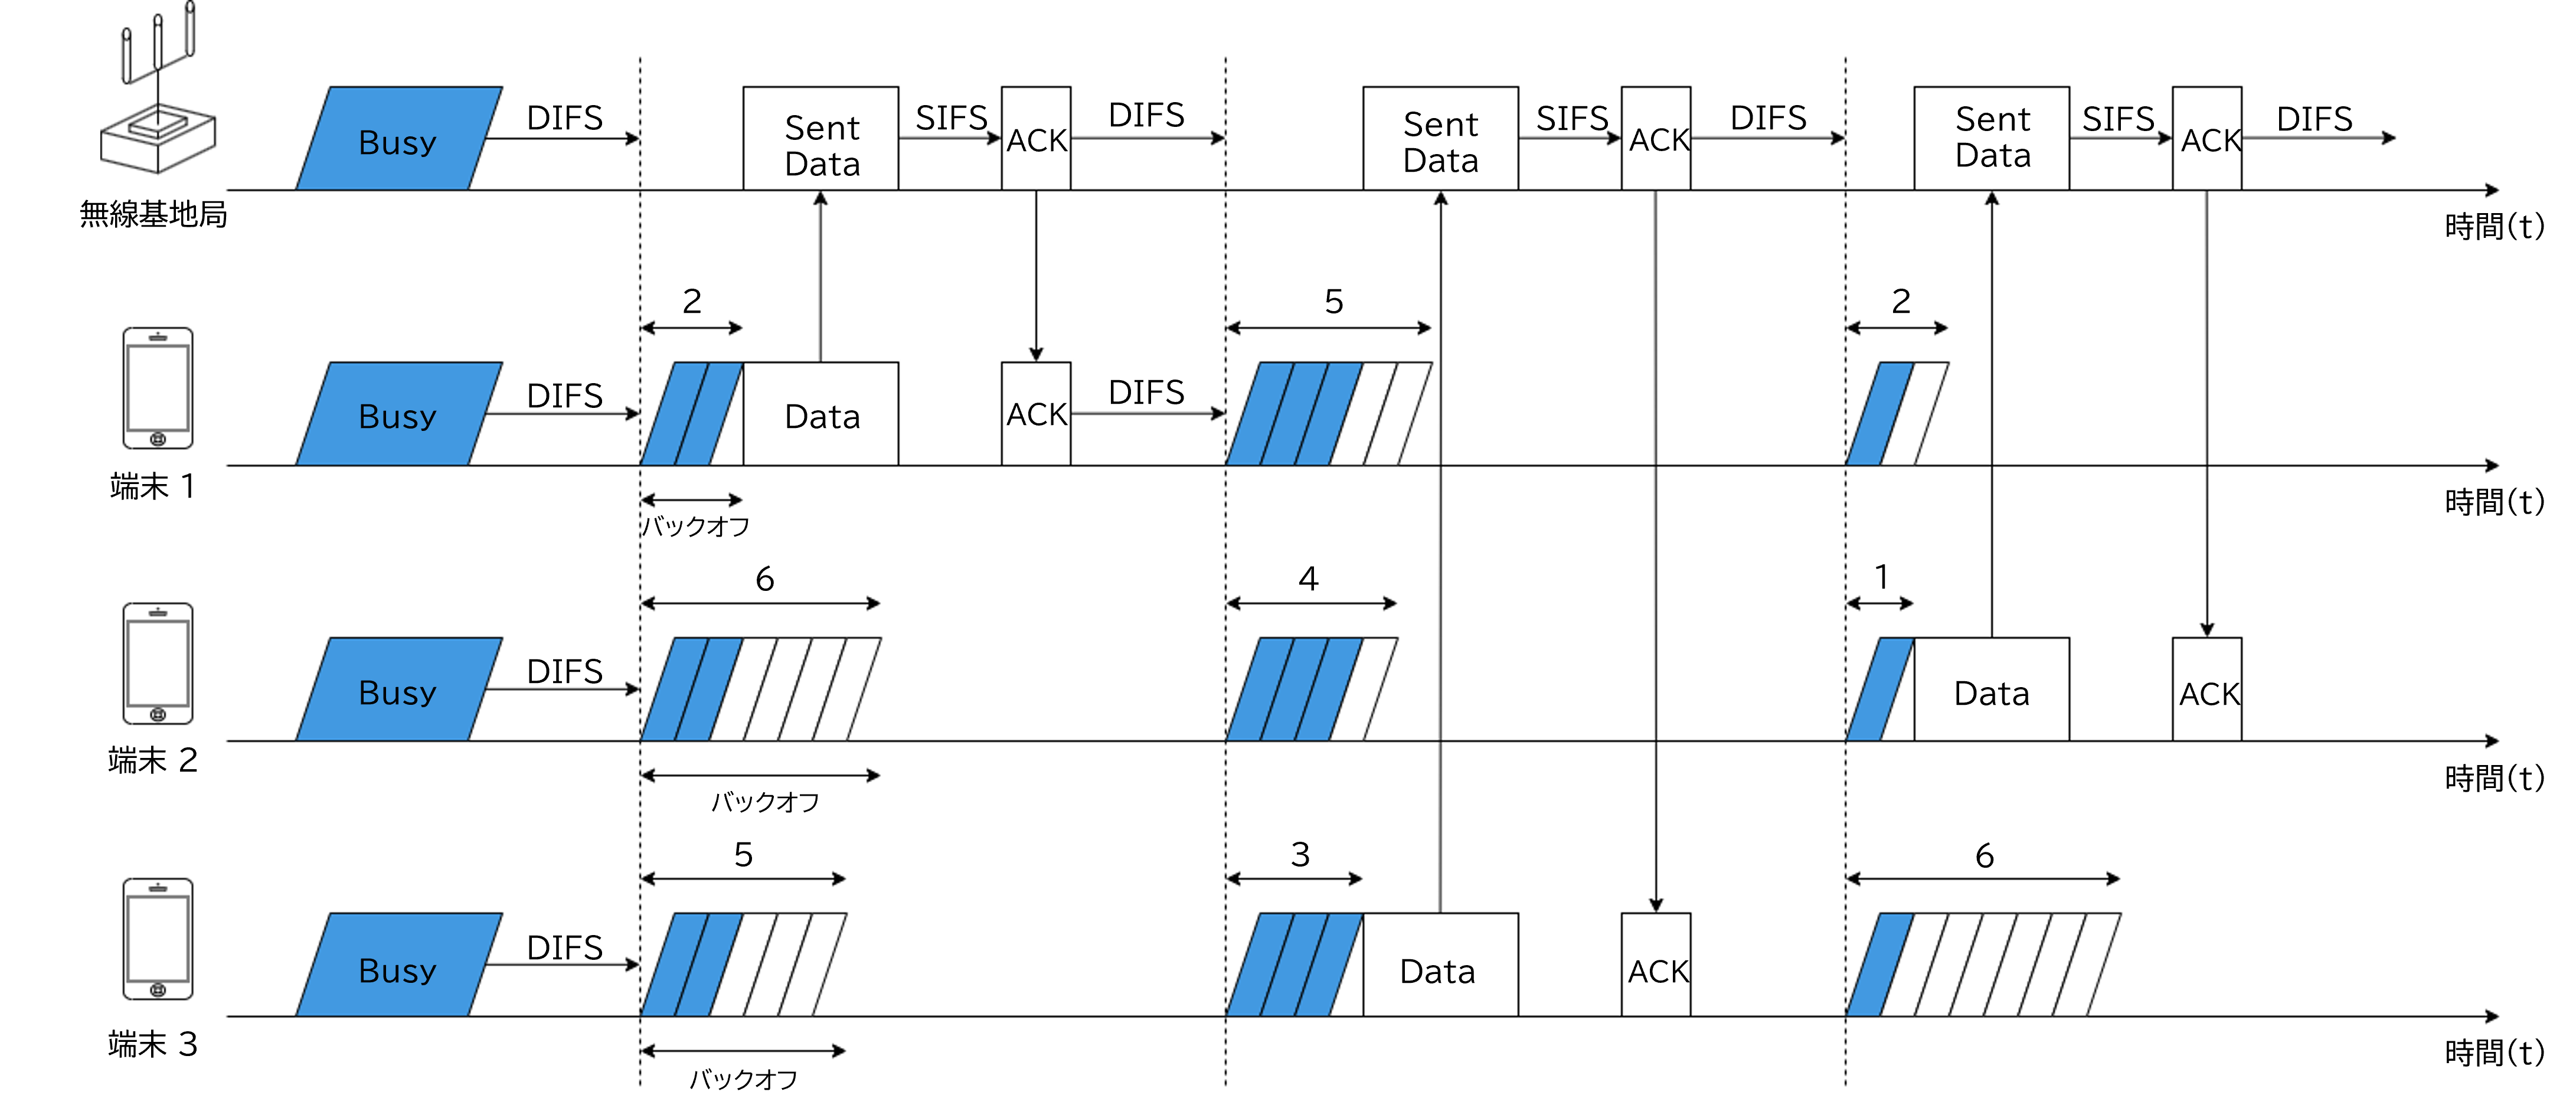
\includegraphics[width=1\textwidth]{./assets/csma-ca-s.png}
    \caption{CSMA/CA成功例}
    \label{1a}
  \end{subfigure}


  \begin{subfigure}{\textwidth}
    \centering
    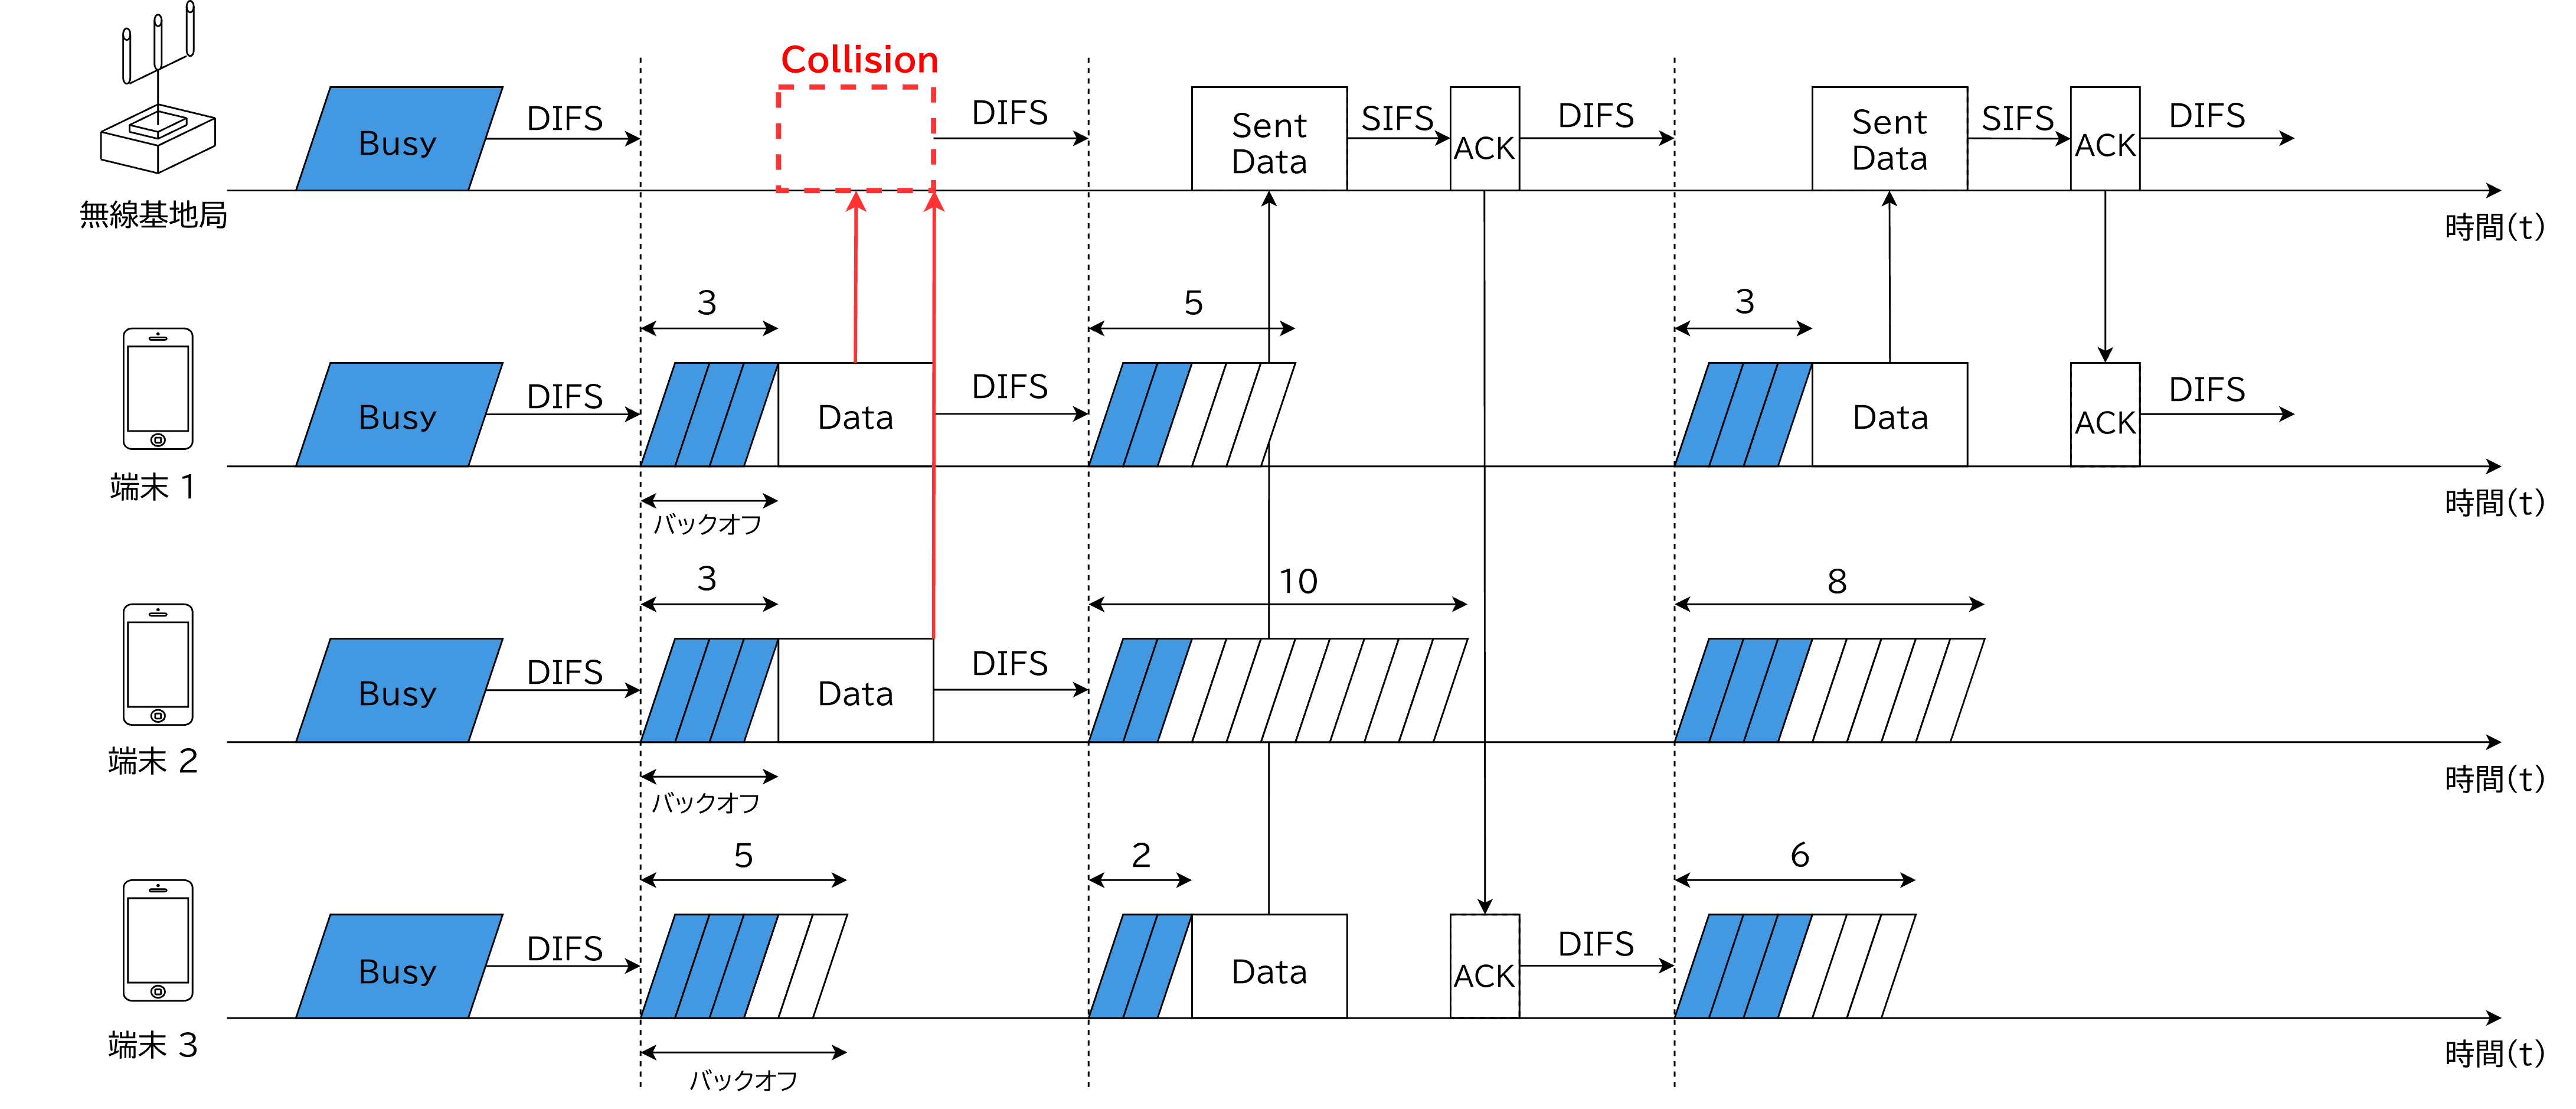
\includegraphics[width=1\textwidth]{./assets/csma-ca-f.png}
    \caption{CSMA/CA失敗例}
    \label{1b}
  \end{subfigure}


  \caption{CSMA/CAの概要}
  \label{CSMA/CA}
\end{figure}


% ******************************************************
% 参考文献
% ******************************************************
\clearpage
\addcontentsline{toc}{section}{参考文献}
\begin{thebibliography}{99}

\bibitem{midori}守倉正博, 久保田周治, 『インプレス標準教科書シリーズ 改訂三版802.11 高速無線LAN教科書』, 株式会社インプレスコミュニケーションズ, 2016年
\bibitem{paper}Y. Morino, T. Hiraguri, H. Yoshino, K. Nishimori, T. Matsuda, ``A Novel Collision Avoidance Scheme Using Optimized Contention Window in Dense Wireless LAN Environments*'' \, \textit{IEICE TRANS. COMMUN.}, VOL.E99-B, NO.11 NOVEMBER 2016
\bibitem{book1}西森健太郎,平栗健史,『MIMOからMassive MIMOを用いた伝送技術とクロスレイヤ評価手法』, コロナ社, 2017年.
\bibitem{book2}設樂勇, 平栗健史, 谷口諒太郎, 西森健太郎, 『レイトレースを用いた3次元クロスレイヤシミュレータの開発』, 社団法人 電子情報通信学会 信学技報

\end{thebibliography}

\end{document}
